Now let's talk about linear classification. Remember that the MSE was a nice loss to choose due to the Gauss-Markov theorem, but is there an analogue for classification? Since we are now working in classification, a natural metric would be to see the proportion of samples we get correct, and this is modeled through the $0$-$1$ loss function. 
\begin{equation}
  L(f, x, y) = \mathbbm{1}(y = f(x))
\end{equation} 
However, this isn't a smooth function to work with, with $0$ gradients almost everywhere and hard to solve analytically. We can try a couple things. 

Alternatively, we can use a \textbf{surrogate loss function} to approximate the 0-1 loss function. The logistic uses some function, and the SVM uses the smallest convex function to approximate the 0-1 loss function. Here are some examples: 

\begin{figure}[H]
  \centering
  \begin{subfigure}[b]{0.48\textwidth}
    \centering
    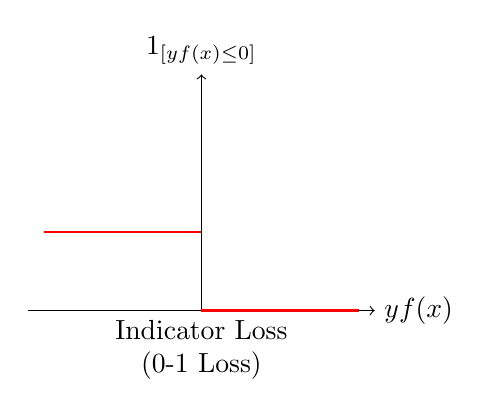
\begin{tikzpicture}
      \draw[->] (-2.2,0) -- (2.2,0) node[right] {$yf(x)$};
      \draw[->] (0,0) -- (0,3) node[above] {$1_{[yf(x)\leq0]}$};
      \draw[red, thick] (-2,1) -- (0,1);
      \draw[red, thick] (0,0) -- (2,0);
      \node[align=center] at (0,-0.5) {Indicator Loss\\(0-1 Loss)};
    \end{tikzpicture}
    \caption{Indicator/0-1 Loss can't be easily optimized.}
    \label{fig:indicator}
  \end{subfigure}
  \begin{subfigure}[b]{0.48\textwidth}
    \centering
    \begin{tikzpicture}
      \draw[->] (-2.2,0) -- (2.2,0) node[right] {$yf(x)$};
      \draw[->] (0,0) -- (0,3) node[above] {$e^{-yf(x)}$};
      \draw[green!50!black, thick, domain=-2:2, samples=100] 
        plot (\x, {0.5*exp(-0.7*\x)});
    \end{tikzpicture}
    \caption{Exponential Loss for Adaboost.}
    \label{fig:exponential}
  \end{subfigure}
  
  \begin{subfigure}[b]{0.48\textwidth}
    \centering
    \begin{tikzpicture}
      \draw[->] (-2.2,0) -- (2.2,0) node[right] {$yf(x)$};
      \draw[->] (0,0) -- (0,3) node[above] {$\log(1+e^{-yf(x)})$};
      \draw[blue, thick, domain=-2:2, samples=100] 
        plot (\x, {ln(1 + exp(-\x))});
    \end{tikzpicture}
    \caption{Log Loss for logistic regression. }
    \label{fig:logistic}
  \end{subfigure}
  \begin{subfigure}[b]{0.48\textwidth}
    \centering
    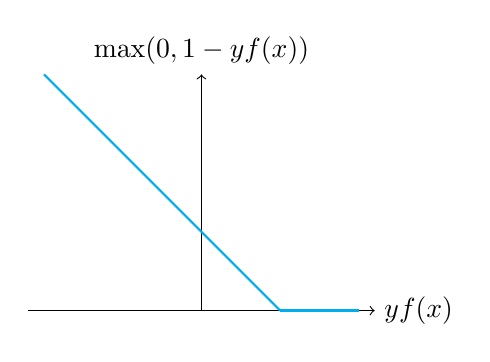
\begin{tikzpicture}
      \draw[->] (-2.2,0) -- (2.2,0) node[right] {$yf(x)$};
      \draw[->] (0,0) -- (0,3) node[above] {$\max(0,1-yf(x))$};
      \draw[cyan, thick] (-2,3) -- (1,0);
      \draw[cyan, thick] (1,0) -- (2,0);
    \end{tikzpicture}
    \caption{Hinge Loss for support vector machines.}
    \label{fig:hinge}
  \end{subfigure}
  \caption{Common loss functions used in classification}
  \label{fig:loss_functions}
\end{figure} 

Intuitively, regression seems like a much harder problem than classification. One predicts over a finite set of values while the other predicts over a continuum. We can try and solve the problem as if we were going regression of values between $0$ and $1$, and then put a cutoff threshold where it classifies $0$ if $f(x) \leq \frac{1}{2}$ and $1$ if else. This is called the \textit{Bayes' classifier}. 

\begin{theorem}[Minimality of Bayes Classifier]
  \label{thm:bayes_optimality}
  The function $f^\ast$ that minimizes the expected risk of the $0$-$1$ loss is 
  \begin{equation}
    f^\ast(x) = \begin{cases} 
      0 & \text{ if } g(x) \leq \frac{1}{2} \\ 
      1 & \text{ if } g(x) > \frac{1}{2} 
    \end{cases}
  \end{equation}
  where $g(x) = \mathbb{E}[Y \mid X = x] = \mathbb{P}(Y = 1 \mid X = x)$ denotes the regression function. 
\end{theorem}
\begin{proof}
  It suffices to show that
  \begin{equation}
    \mathbb{P}(Y \neq h(X)|X = x) - \mathbb{P}(Y \neq h^*(X)|X = x) \geq 0 \quad \text{for all } x \in \mathcal{X}.
  \end{equation}
  
  Now,
  \begin{align}
    \mathbb{P}(Y \neq h(X)|X = x) &= 1 - \mathbb{P}(Y = h(X)|X = x) \\
    &= 1 - \left(\mathbb{P}(Y = 1, h(X) = 1|X = x) + \mathbb{P}(Y = 0, h(X) = 0|X = x)\right) \\
    &= 1 - \left(h(x)\mathbb{P}(Y = 1|X = x) + (1 - h(x))\mathbb{P}(Y = 0|X = x)\right) \\
    &= 1 - \left(h(x)m(x) + (1 - h(x))(1 - m(x))\right).
  \end{align}
  
  Hence,
  \begin{align}
    &\mathbb{P}(Y \neq h(X)|X = x) - \mathbb{P}(Y \neq h^*(X)|X = x) \\
    &= \left(h^*(x)m(x) + (1 - h^*(x))(1 - m(x))\right) - \left(h(x)m(x) + (1 - h(x))(1 - m(x))\right) \\
    &= (2m(x) - 1)(h^*(x) - h(x)) = 2\left(m(x) - \frac{1}{2}\right)(h^*(x) - h(x)) \label{res}
  \end{align}
  
  When $m(x) \geq 1/2$ and $h^*(x) = 1$, \eqref{res} is non-negative. When $m(x) < 1/2$ and $h^*(x) = 0$, \eqref{res} is again non-negative. 
\end{proof}

In fact, by fitting a regression function over any data, we can simply compose it with the threshold function to get a binary classifier. This is called the \textbf{plug-in classifier}. 

\begin{definition}[Plug-In Classifier]
  Given an regression estimator $\hat{g}$, we can define the corresponding \textbf{plug-in classifier} as 
  \begin{equation}
    \hat{f}(x) = \begin{cases} 
      0 & \text{ if } \hat{g}(x) \leq \frac{1}{2} \\ 
      1 & \text{ if } \hat{g}(x) > \frac{1}{2} 
    \end{cases}
  \end{equation}
\end{definition}

Due to the optimality of the Bayes' classifier, the performance of the plug-in classifier is tied to the performance of the underlying linear regression model. We can actually formalize this with the following. 

\begin{theorem}[Classification Risk Bounded by Regression Risk]
  The risk of the plug-in classifier rule in (14) satisfies
  \begin{equation}
    R(\hat{h}) - R^\ast \leq 2\sqrt{\int (\hat{m}(x) - m^\ast(x))^2 dP_X(x)}.
  \end{equation}
\end{theorem}
\begin{proof}
  In the proof of \href{thm:bayes_optimality}{the previous theorem} we showed that
  \begin{align}
    \mathbb{P}(Y \neq \hat{h}(X)|X = x) 
    & - \mathbb{P}(Y \neq h^{\ast}(X)|X = x) \\ 
    & = (2\hat{m}(x) - 1)(h^{\ast}(x) - \hat{h}(x)) \\
    & = |2\hat{m}(x) - 1|I(h^{\ast}(x) \neq \hat{h}(x)) \\ 
    & = 2|\hat{m}(x) - 1/2|I(h^{\ast}(x) \neq \hat{h}(x)).
  \end{align}
  
  Now, when $h^{\ast}(x) \neq \hat{h}(x)$, there are two possible cases: (i) $\hat{h}(x) = 1$ and $h^{\ast}(x) = 0$; (ii) $\hat{h}(x) = 0$ and $h^{\ast}(x) = 1$. In both cases, we have that $|\hat{m}(x) - m^{\ast}(x)| \geq |\hat{m}(x) - 1/2|$. Therefore,
  \begin{align}
    \mathbb{P}(\hat{h}(X) \neq Y) - \mathbb{P}(h^{\ast}(X) \neq Y) &= 2\int |\hat{m}(x) - 1/2|I(h^{\ast}(x) \neq \hat{h}(x))dP_X(x) \\
    &\leq 2\int |\hat{m}(x) - m^{\ast}(x)|I(h^{\ast}(x) \neq \hat{h}(x))dP_X(x) \\
    &\leq 2\int |\hat{m}(x) - m^{\ast}(x)|dP_X(x) \tag{15} \\
    &\leq 2\sqrt{\int (\hat{m}(x) - m^{\ast}(x))^2 dP_X(x)}. \tag{16}
  \end{align}
  
  The last inequality follows from the fact that $\mathbb{E}|Z| \leq \sqrt{\mathbb{E}Z^2}$ for any $Z$.
\end{proof}
